\chapter{Zeichenerkennung}
\section{Motivation}
Die Idee war es, dass mit dem Lichtsensor Zeichen erkannt werden sollen. Als Zeichen haben wir uns für ein Kreuz, ein Quadrat, ein Dreieck und einen Kreis. Alle Zeichen sind ausgefüllt.

\section{Aufgabenstellung}
Der Roboter soll nur mit Hilfe des Lichtsensors die vier Zeichen erkennen können. Die Zeichen befinden sich in einem umrahmten Feld. Der Abstand eines jeden Zeichens zum Rahmen ist gleich. Die Zeichen und der Rahmen sind schwarz, der Hintergrund ist weiß.

\begin{capfigure}[Symbole der Zeichenerkennung]
	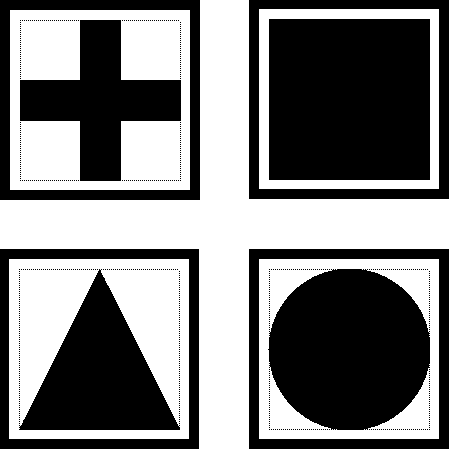
\includegraphics[width=10cm]{images/zeichen/combo}
\end{capfigure}

\section{Lösung}

Bei der Lösung haben wir uns für die Variante mit einem Lichtsensor entschieden. Wie fahren einmal ab und messen das Verhältnis der beiden weißen Abschnitte und des schwarzen Abschnitts. Anhand dessen kann entschieden werden um welches Zeichen es sich handelt.

Die Lösung ist auf der DVD unter \textit{Lösungen/Zeichenerkennung} zu finden.